% Fig. 1 — Modelo de interacción multicapa S = (O, K, M, D).
% Figura vectorial nativa en TikZ (fuente reutilizable en el paper LaTeX).
% Compilar: pdflatex fig1_modelo_multicapa.tex  -> fig1_modelo_multicapa.pdf
% Sin título embebido (INV-12): el título va en el \caption del paper.
\documentclass[border=6pt]{standalone}
\usepackage[utf8]{inputenc}
\usepackage[T1]{fontenc}
\usepackage{lmodern}
\usepackage{tikz}
\usetikzlibrary{arrows.meta, positioning}
\begin{document}
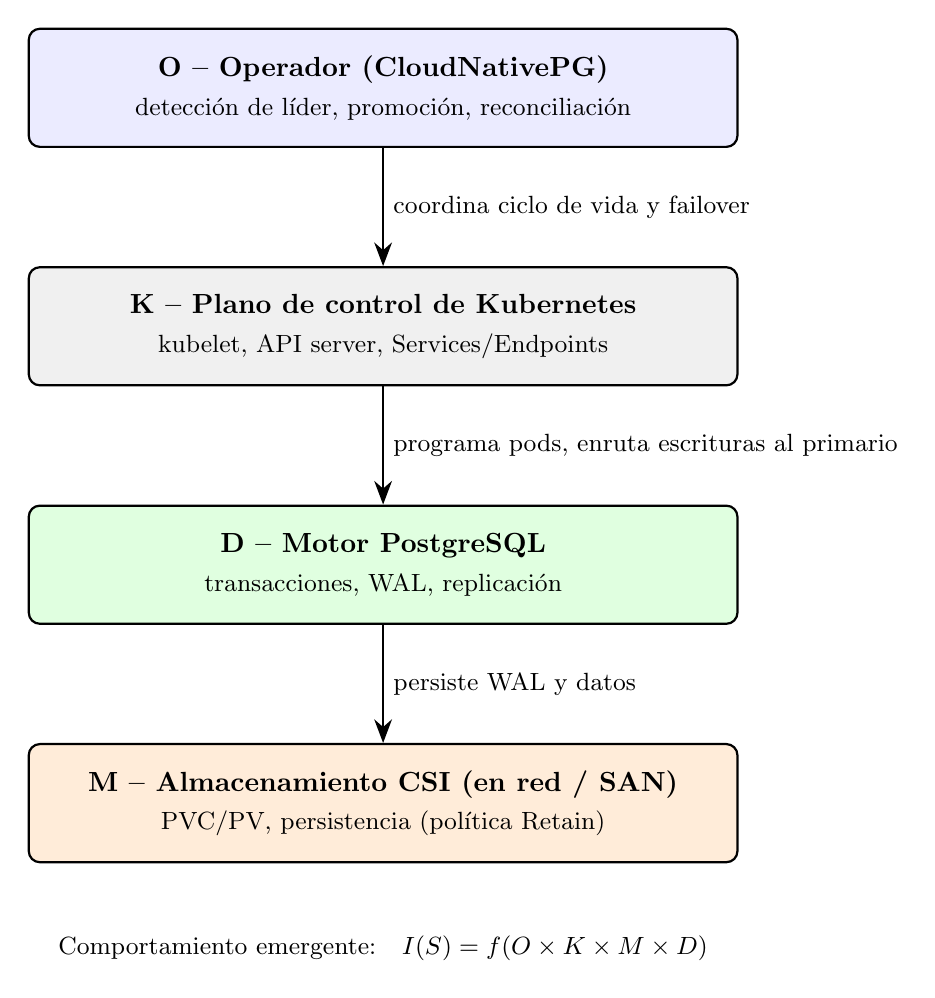
\begin{tikzpicture}[
  layer/.style={draw, rounded corners, minimum width=9cm, minimum height=1.5cm, align=center, thick},
  flow/.style={-{Stealth[length=3mm]}, thick},
  lbl/.style={font=\small}
]
  \node[layer, fill=blue!8]                    (O) {\textbf{O -- Operador (CloudNativePG)}\\[2pt]\small detección de líder, promoción, reconciliación};
  \node[layer, fill=black!6, below=1.5cm of O] (K) {\textbf{K -- Plano de control de Kubernetes}\\[2pt]\small kubelet, API server, Services/Endpoints};
  \node[layer, fill=green!12, below=1.5cm of K](D) {\textbf{D -- Motor PostgreSQL}\\[2pt]\small transacciones, WAL, replicación};
  \node[layer, fill=orange!15, below=1.5cm of D](M){\textbf{M -- Almacenamiento CSI (en red / SAN)}\\[2pt]\small PVC/PV, persistencia (política Retain)};
  \draw[flow] (O) -- node[right, lbl] {coordina ciclo de vida y failover} (K);
  \draw[flow] (K) -- node[right, lbl] {programa pods, enruta escrituras al primario} (D);
  \draw[flow] (D) -- node[right, lbl] {persiste WAL y datos} (M);
  \node[below=0.8cm of M, font=\small] {Comportamiento emergente:\quad $I(S) = f(O \times K \times M \times D)$};
\end{tikzpicture}
\end{document}
